\section{\Large SPECIFICATIONS}
\subsection{Requirements}
NISAR is a joint Earth-observation satellite mission between NASA and ISRO. It is the first satellite to operate in two different Synthetic Aperture Radar (SAR) bands, incorportating both L- and S-band SAR instruments. Both frequencies can penetrate clouds for reliable data collection, but the L-band can also penetrate thicker vegetation that the S-band cannot. Uniquely, NISAR is intended to be used for a wide range of science objectives, including disaster response and agriculture \cite{NISARApps}.

NISAR ADCS requirements are \textless 273 arcseconds for pointing and \textless 500 m for orbit control \cite{Siqueira}. The satellite duty cycle is specified as \textgreater 30\%. NISAR will operate in LEO with nominal altitude of 747 km and 6 AM/6 PM orbit. NISAR's L- and S-band instruments operate at 24 cm and 12 cm wavelengths, respectively. NISAR collects terrestial SAR imagery with an image swatch of 240 km using a sweep approach. The science payload can also perform polarimetry, with the SAR incorporating multiple polarization modes.

\subsection{Layout}
\begin{figure}[H]
\centering
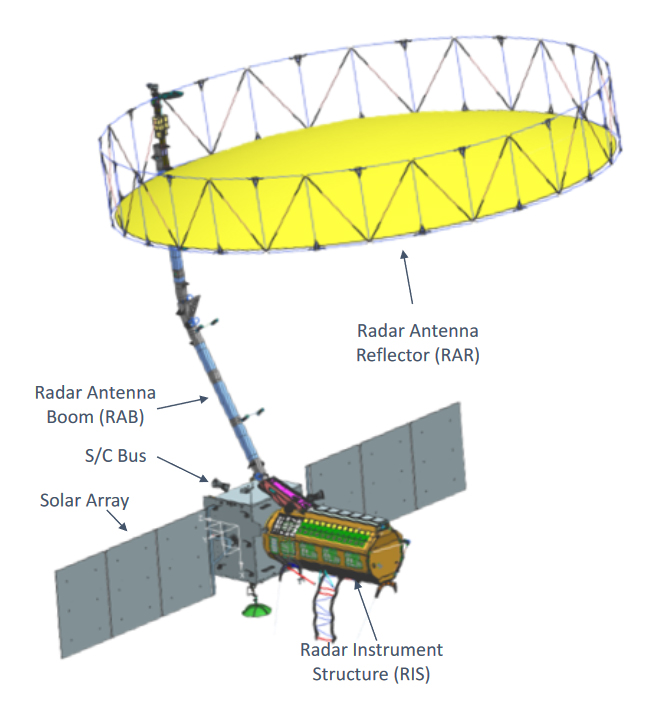
\includegraphics[scale=0.38]{Images/nisar_diagram.jpg}
\caption{The basic components of the NISAR satellite}
\label{NISAR Diagram}
\end{figure}

As shown in Figure \ref{NISAR Diagram}, NISAR's satellite consists of a 1.2 m x 1.8 m x 1.9 m spacecraft bus cuboid with a 1.2 m wide octagonal Radar Instrument Structure (RIS). The spacecraft bus includes ADCS hardware, power subsystem, and engineering payload, while the RIS houses hardware for the L- and S-band SAR. The satellite is powered by 23 m\textsuperscript{2} of solar panels, consisting of an array of two panels, one on each side of the satellite. Additionally, a 12 m diameter radar antenna is positioned above the body of the spacecraft, attached by a 9 m long boom. This boom consists of beams with 7 in x 7 in cross-section area \cite{NISARMission}.

Table \ref{tab:mass} contains mass properties of the satellite. Unfortunately, detailed mass distribution and inertia properties of NISAR are not openly available, so we provide estimates of mass distribution based on known overall component-level masses. We are given total masses for the bus structure and RIS, and we also know the masses of the payloads located within, allowing us to compute an accurate mass for these components \cite{NISARMission}. We estimate that solar panels have a mass of 23 kg each based on knowledge that NISAR's solar panels are 23 m\textsuperscript{2} and a typical solar panel mass per area is 2.06 kg/m\textsuperscript{2} \cite{SolarPanelMass}. We know that the entire radar antenna assembly has a mass of 292 kg, and we estimate that the reflector has a mass of approximately 100 kg based on a similar deployable SAR S- and L-band mesh antenna reflector \cite{L3Harris}. We will use these masses to compute center of mass and moments of inertia in the following section. For our model, we neglect the effects of the truss structure supporting the antenna reflector, instead modeling the entire RAR as just the disk-shaped reflector mesh.

\begin{longtable}{l|r}
\caption{Mass of NISAR components}
\label{tab:mass}\\
\textbf{Components}              & \multicolumn{1}{l}{\textbf{Mass [kg]}} \\ \hline
\endfirsthead
%
\endhead
%
Bus                              & 964.1                                      \\
Radar Instrument Structure (RIS) & 1375.9                                     \\
Solar Panel +y                   & 23                                         \\
Solar Panel -y                   & 23                                         \\
Radar Antenna Boom (RAB)         & 192                                        \\
Radar Antenna Reflector (RAR)    & 100                                       
\end{longtable}

Since NISAR is a remote sensing satellite requiring high attitude control performance, it has an ADCS system with an array of sensors and actuators. Sensors include star sensors, sun sensors, GPS, and a 3-axis gyroscope for roll, pitch, and yaw. For actuators, NISAR has four 50 N$\cdot$m reaction wheels mounted in tetrahedral configuration, three 565 and 350 A$\cdot$m\textsuperscript{2} magnetorquers, and fourteen thrusters (ten canted 11 N thrusters, one central 11 N thruster, and four 1 N thrusters for roll) \cite{NISARMission}.

\subsection{Mass Properties}
We simplify the spacecraft geometry into six components, each individually assumed to have uniform mass distribution. These components of the simplified geometry are: bus structure (including ADCS hardware and engineering payload), RIS (Radar Instrument Structure), RAB (radar antenna boom), RAR (radar antenna reflector), and two solar panels (identified as the +y solar panel and -y solar panel). The bus structure is modeled as a rectangular prism, while the RIS is modeled as an octagonal prism. The RAB is also modeled as a rectangular prism, while the RAR is modeled as a thin disk and the solar panels are modeled as thin rectangular plates. Within each geometry, our model assumes mass is distributed uniformly. From analyzing diagrams found in technical reports, we estimate that the RAR is tilted -3.87\degree{} about the y-axis (relative to the x-axis), while the RAB is modeled as a single beam with an angle approximately -18\degree{} from vertical (from the z-axis, about the y-axis in the x-z plane). Note that we have simplified the shape of the RAB from a beam of two angled segments to a single, straight beam.

We choose the body axes to have an origin at the center of the rectangular bus. This configuration is chosen because the bus houses the ADCS hardware, including actuators and sensors. The x-axis points in the direction of the RIS, and the z-axis points up vertically, normal to the upper surface of the bus. See Figure \ref{fig:MATLAB_model} for a visual depiction of the body axes relative to the spacecraft.

We compute the center of mass after extracting the centroid of each component. The mass of each component is previously found in Table \ref{tab:mass}. The centroid of each component is listed in Table \ref{tab:centroid}.

\begin{longtable}{l|r|r|r}
\caption{Component centroids [m]}
\label{tab:centroid}\\
\textbf{Part} & \multicolumn{1}{l}{\textbf{x}} & \multicolumn{1}{l}{\textbf{y}} & \multicolumn{1}{l}{\textbf{z}} \\ \hline
\endfirsthead
%
\endhead
%
Bus      & 0     & 0    & 0    \\
RIS      & 1.85  & 0    & 0    \\
Panel +y & 0     & 3.9  & 0    \\
Panel -y & 0     & -3.9 & 0    \\
RAB      & -0.899 & 0    & 5.194 \\
RAR      & 4.283   & 0    & 8.308
\end{longtable}

The center of mass can be found by taking the weighted average of each component centroid, weighted by the mass of each component. The center of mass formula is:
\begin{equation*}
    \Vec{r}_{cm} = \frac{\sum m_{i} \Vec{r}_{i}}{\sum m_{i}}
\end{equation*}
This yields a result for center of mass at $\qty[parse-numbers = false]{[1.046, 0, 0.683]}{\metre}$ relative to the origin we defined. We use a MATLAB script to compute the center of mass from a CSV file containing centroid and mass data.

We compute the moment of inertia of the satellite, finding an inertia tensor in our body axes. To do this, we break the satellite into individual components, first finding the moment of inertia about the center of mass of each component. We then compute the moment of inertia of the entire satellite about the body axes by using parallel axis theorem and combining all the components.

To compute the moment of inertia, we need the following geometric properties of each component:

\begin{longtable}{l|r|r|r|r|r}
\caption{Dimensions of modeled components [m]}
\label{tab:dimensions}\\
\textbf{Part} & \textbf{L (x-dim)} & \textbf{W (y-dim)} & \textbf{H (z-dim)} & \textbf{S (oct. side length)} & \textbf{R (radius)} \\ \hline
\endfirsthead
%
\endhead
%
Bus &  & 1.8 & 1.9 & - & - \\
RIS & 2.5 & - & - & 0.459 & - \\
Panel +y & - & 6 & 1.9 & - & - \\
Panel -y & - & 6 & 1.9 & - & - \\
RAB & 0.1778 & 0.1778 & 9 & - & - \\
RAR & - & - & - & - & 6
\end{longtable}

For the bus, we choose to model the geometry as a rectangular prism. Since the bus is aligned with the body axes, we obtain a diagonal inertia tensor:
\begin{align*}
I_{bus} &=
\begin{bmatrix}
I_{xx} & 0 & 0 \\
0 & I_{yy} & 0 \\
0 & 0 & I_{zz}
\end{bmatrix} \\
&=
\begin{bmatrix}
m \frac{W^{2} + H^{2}}{12} & 0 & 0 \\
0 & m \frac{L^{2} + H^{2}}{12} & 0 \\
0 & 0 & m \frac{L^{2} + W^{2}}{12} 
\end{bmatrix} \\
&=
\qty[parse-numbers = false]{
\begin{bmatrix}
550.340 & 0 & 0 \\
0 & 405.725 & 0 \\
0 & 0 & 375.9993 
\end{bmatrix}
}{\kilogram\metre\squared}
\end{align*}
For the solar panels, we approximate their geometry as a flat plate. These axes are also aligned, so the tensor can be diagonal.
\begin{align*}
I_{panel} &=
\begin{bmatrix}
I_{xx} & 0 & 0 \\
0 & I_{yy} & 0 \\
0 & 0 & I_{zz}
\end{bmatrix} \\
&=
\begin{bmatrix}
m \frac{W^{2} + H^{2}}{12} & 0 & 0 \\
0 & m \frac{H^{2}}{12} & 0 \\
0 & 0 & m \frac{W^{2}}{12} 
\end{bmatrix} \\
&=
\qty[parse-numbers = false]{
\begin{bmatrix}
75.919 & 0 & 0 \\
0 & 6.919 & 0 \\
0 & 0 & 69 
\end{bmatrix}
}{\kilogram\metre\squared}
\end{align*}
For the RIS, we model the geometry as an octagonal prism. For the moment of inertia about the axisymmetric axis of the octagon, we use the formula $m \left(\frac{S^{2}}{24} + \frac{a^{2}}{2}\right)$, where $S$ is the side length and $a$ is the apothem length, where the apothem is the perpendicular length from a side of the octagon to the center \cite{McCarron}. When calculating the moment of inertia about the non-axisymmetric axes, we approximate the geometry as a cylinder with radius equal to the average of the octagonal radius (distance from center to vertex) and the apothem. As will be shown later, this approximation yields a very close result to the inertia tensor generated from the CAD model.
\begin{align*}
I_{RIS} &=
\begin{bmatrix}
I_{xx} & 0 & 0 \\
0 & I_{yy} & 0 \\
0 & 0 & I_{zz}
\end{bmatrix} \\
&=
\begin{bmatrix}
m \left(\frac{S^{2}}{24} + \frac{a^{2}}{2}\right) & 0 & 0 \\
0 & m \left(\frac{L^{2}}{12} + \frac{R_{avg}^{2}}{4}\right) & 0 \\
0 & 0 & m \left(\frac{L^{2}}{12} + \frac{R_{avg}^{2}}{4}\right) 
\end{bmatrix} \\
&=
\qty[parse-numbers = false]{
\begin{bmatrix}
223.268 & 0 & 0 \\
0 & 831.089 & 0 \\
0 & 0 & 831.089 
\end{bmatrix}
}{\kilogram\metre\squared}
\end{align*}
For the RAB, we first model the geometry as a rectangular prism. We also must rotate the inertia tensor to match the orientation of the body axes, as the RAB itself is rotated relative to the bus about the y-axis by -18\degree{} from vertical (z-axis).
\begin{align*}
I_{RAB} &=
\begin{bmatrix}
I_{xx} & 0 & 0 \\
0 & I_{yy} & 0 \\
0 & 0 & I_{zz}
\end{bmatrix} \\
&=
\begin{bmatrix}
m \frac{W^{2} + H^{2}}{12} & 0 & 0 \\
0 & m \frac{L^{2} + H^{2}}{12} & 0 \\
0 & 0 & m \frac{L^{2} + W^{2}}{12} 
\end{bmatrix} \\
&=
\qty[parse-numbers = false]{
\begin{bmatrix}
1296.506 & 0 & 0 \\
0 & 1296.506 & 0 \\
0 & 0 & 1.012 
\end{bmatrix}
}{\kilogram\metre\squared}
\end{align*}
We apply the rotation to the inertia tensor using a rotation matrix about the y-axis. Note that doing so results in non-zero products of inertia, meaning our principal axes will not be aligned with our body axes.
\begin{align*}
I_{RAB,rotated} &= R_{y}(-18\degree) I_{RAB} R_{y}^{\intercal}(-18\degree) \\
&=
\qty[parse-numbers = false]{
\begin{bmatrix}
1172.797 & 0 & 380.736 \\
0 & 1296.506 & 0 \\
380.736 & 0 & 124.720
\end{bmatrix}
}{\kilogram\metre\squared}
\end{align*}
Finally, we model the RAR as a flat disk. Similar to the RAB, we must rotate the inertia tensor to match the orientation of the body axes.
\begin{align*}
I_{RAR} &=
\begin{bmatrix}
I_{xx} & 0 & 0 \\
0 & I_{yy} & 0 \\
0 & 0 & I_{zz}
\end{bmatrix} \\
&=
\begin{bmatrix}
m \frac{R^{2}}{4} & 0 & 0 \\
0 & m \frac{R^{2}}{4} & 0 \\
0 & 0 & m \frac{R^{2}}{2} 
\end{bmatrix} \\
&=
\qty[parse-numbers = false]{
\begin{bmatrix}
900 & 0 & 0 \\
0 & 900 & 0 \\
0 & 0 & 1800 
\end{bmatrix}
}{\kilogram\metre\squared}
\end{align*}
Applying a rotation:
\begin{align*}
I_{RAR,rotated} &= R_{y}(-3.87\degree) I_{RAR} R_{y}^{\intercal}(-3.87\degree) \\
&=
\qty[parse-numbers = false]{
\begin{bmatrix}
904.100 & 0 & -60.605 \\
0 & 900 & 0 \\
-60.605 & 0 & 1795.900
\end{bmatrix}
}{\kilogram\metre\squared}
\end{align*}
Now, we use parallel axis theorem to compute the moment of inertia of each component about the body axes at the specified origin. We can use the following displacement tensor,
\begin{equation*}
D =
\begin{bmatrix}
y^{2} + z^{2} & -xy & -xz \\
-yx & x^{2} + z^{2} & -yz \\
-zx & -yz & x^{2} + y^{2}
\end{bmatrix},
\end{equation*}
where $x$, $y$, $z$ are the coordinates of the center of mass of the component, giving the moment of inertia about a new point:
\begin{equation*}
    I' = I_{c} + mD
\end{equation*}
Performing the parallel axis theorem on each component and summing the inertia tensors, we obtain the following inertia tensor for the entire spacecraft:
\begin{equation*}
I_{NISAR,body} =
\qty[parse-numbers = false]{
\begin{bmatrix}
15783.996 & 0 & -2341.659 \\
0 & 22227.752 & 0 \\
-2341.659 & 0 & 10663.970
\end{bmatrix}
}{\kilogram\metre\squared}
\end{equation*}
Compare this with the inertia tensor computed by SolidWorks CAD software:
\begin{equation*}
I_{NISAR,body} =
\qty[parse-numbers = false]{
\begin{bmatrix}
15780.361 & 0 & -2336.285 \\
0 & 22225.721 & 0 \\
-2336.285 & 0 & 10665.796
\end{bmatrix}
}{\kilogram\metre\squared}
\end{equation*}
The errors are 0.0230\%, 0.00914\%, 0.0171\%, and 0.230\% for $I_{xx}$, $I_{yy}$, $I_{zz}$, and $I_{xz}$, respectively. We created the following MATLAB script to compute the inertia tensor.

\subsection{Surface Properties}
For the purpose of discretizing the spacecraft into surfaces, we consider the outer faces of the bus, RIS, and RAB. We also consider the faces of the solar panels and RAR, which are modeled as thin plates. The centroid (barycenter) coordinates and area for each surface are obtained using the surface properties tool in SolidWorks, and a unit normal vector is manually computed based on the orientation of the surface. We then enter this data into a CSV file, which can be read into MATLAB.

This function stores the data into arrays of barycenter coordinates, unit normal vector components, and area. Each row of an array corresponds to a particular surface. The data is shown in Table \ref{tab:surfaces}, annotated with the identity of each surface.

\begin{longtable}{l|r|r|r|r|r|r|r}
\caption{Surface parameters}
\label{tab:surfaces}\\
 &
  \multicolumn{3}{c}{\textbf{Barycenter [m]}} &
  \multicolumn{3}{c}{\textbf{Normal}} &
  \multicolumn{1}{l}{} \\
\endfirsthead
%
\endhead
%
\textbf{Surface} &
  \multicolumn{1}{l}{\textbf{x}} &
  \multicolumn{1}{l}{\textbf{y}} &
  \multicolumn{1}{l}{\textbf{z}} &
  \multicolumn{1}{l}{\textbf{x}} &
  \multicolumn{1}{l}{\textbf{y}} &
  \multicolumn{1}{l}{\textbf{z}} &
  \multicolumn{1}{l}{\textbf{Area [m\textsuperscript{2}]}} \\ \hline
Bus front, minus RIS (+x) & 0.6   & 0     & 0     & 1      & 0      & 0      & 2.4   \\
Bus rear (-x)                  & -0.6  & 0     & 0     & -1     & 0      & 0      & 3.42  \\
Bus side (+y)                  & 0     & 0.9   & 0     & 0      & 1      & 0      & 2.28  \\
Bus side (-y)                  & 0     & -0.9  & 0     & 0      & -1     & 0      & 2.28  \\
Bus top (+z)                   & 0     & 0     & 0.95  & 0      & 0      & 1      & 2.16  \\
Bus bottom (-z)                & 0     & 0     & -0.95 & 0      & 0      & -1     & 2.16  \\
RIS front (+x)                 & 3.1   & 0     & 0     & 1      & 0      & 0      & 1.02  \\
RIS top (+z)                   & 1.85  & 0     & 0.55  & 0      & 0      & 1      & 1.15  \\
RIS bottom (-z)                & 1.85  & 0     & -0.55 & 0      & 0      & -1     & 1.15  \\
RIS side (+y)                  & 1.85  & 0.55  & 0     & 0      & 1      & 0      & 1.15  \\
RIS side (-y)                  & 1.85  & -0.55 & 0     & 0      & -1     & 0      & 1.15  \\
RIS angle face (y-z I)         & 1.85  & 0.39  & 0.39  & 0      & 0.707  & 0.707  & 1.15  \\
RIS angle face (y-z II)        & 1.85  & -0.39 & 0.39  & 0      & -0.707 & 0.707  & 1.15  \\
RIS angle face (y-z III)       & 1.85  & -0.39 & -0.39 & 0      & -0.707 & -0.707 & 1.15  \\
RIS angle face (y-z IV)        & 1.85  & 0.39  & -0.39 & 0      & 0.707  & -0.707 & 1.15  \\
Panel +y front (+x)            & 0     & 3.9   & 0     & 1      & 0      & 0      & 11.4  \\
Panel +y rear (-x)             & 0     & 3.9   & 0     & -1     & 0      & 0      & 11.4  \\
Panel -y front (+x)            & 0     & -3.9  & 0     & 1      & 0      & 0      & 11.4  \\
Panel -y rear (-x)             & 0     & -3.9  & 0     & -1     & 0      & 0      & 11.4  \\
RAB front (x-z, +x)            & -0.81 & 0     & 5.21  & 0.951  & 0      & 0.309  & 1.6   \\
RAB rear (x-z, -x)             & -0.99 & 0     & 5.18  & -0.951 & 0      & -0.309 & 1.6   \\
RAB side (+y)                  & -0.9  & -0.09 & 5.19  & 0      & 1      & 0      & 1.6   \\
RAB side (-y)                  & -0.9  & 0.09  & 5.19  & 0      & -1     & 0      & 1.6   \\
RAB top (+z)                   & -2.31 & 0     & 9.47  & 0      & 0      & 1      & 0.03  \\
RAR top (+z)                   & 4.28  & 0     & 8.31  & -0.067 & 0      & 0.998  & 113.1 \\
RAR bottom (-z)                & 4.28  & 0     & 8.31  & 0.067  & 0      & -0.998 & 113.1
\end{longtable}

\subsection{Body Axes}
A 3D model of the spacecraft is shown in Figure \ref{fig:complex_model}. The model shown is a screen capture from the SolidWorks CAD software.

\begin{figure}[H]
\centering
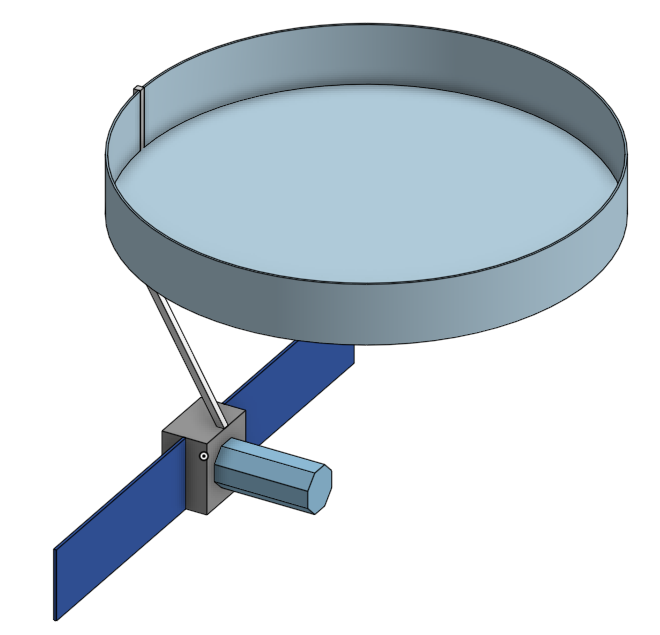
\includegraphics[scale=0.4]{Images/ps1_complex_model.png}
\caption{A 3D model of the satellite}
\label{fig:complex_model}
\end{figure}


We also show a simplified model of the spacecraft in Figure \ref{fig:simple_model}. This is the model we use to compute our mass and surface properties.

\begin{figure}[H]
\centering
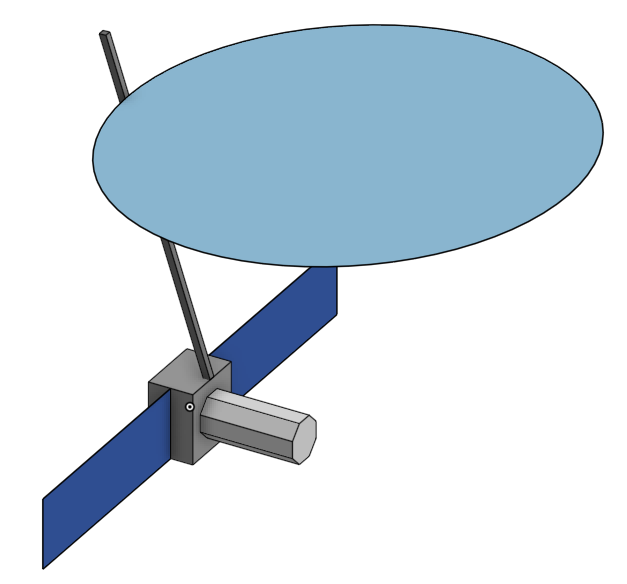
\includegraphics[scale=0.4]{Images/ps1_simple_model.png}
\caption{A 3D model of the simplified satellite geometry}
\label{fig:simple_model}
\end{figure}

We also plot the model in MATLAB by importing an STL version of the CAD model. We show the body axes in Figure \ref{fig:MATLAB_model}, with the origin chosen as the center of the spacecraft bus.

\begin{figure}[H]
\centering
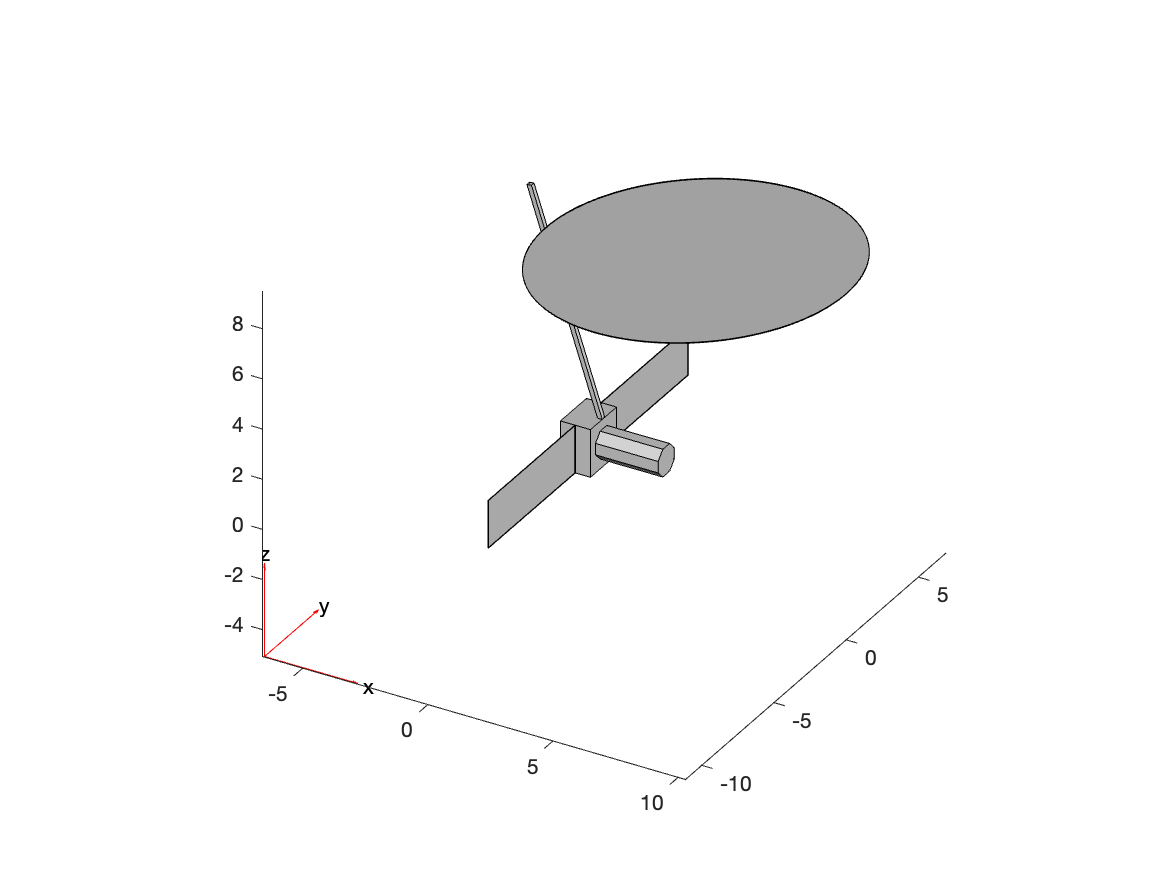
\includegraphics[scale=0.7]{Images/ps1_model.png}
\caption{Satellite model in MATLAB with body axes shown}
\label{fig:MATLAB_model}
\end{figure}

\subsection{Principal Axes}
The unit vectors of the principal axes with respect to the body axes ($\Vec{e}_i$) and the inertia tensor in the principal axes ($I_i$) can be found by taking the eigenvalue decomposition of the inertia tensor in the body axis. This can be seen in the two equations below.
\begin{equation*}
    I_i \cdot \Vec{e}_i = I_i \cdot \Vec{I}_{body} \\ \hspace{1cm} i = x, y, z
\end{equation*}
\begin{align*}
\Vec{I}_{principal} &= 
    \begin{bmatrix}
    I_x & 0 & 0 \\
    0 & I_y & 0 \\
    0 & 0 & I_z 
    \end{bmatrix}
= 
\qty[parse-numbers = false]{
    \begin{bmatrix}
    7707.07 & 0 & 0 \\
    0 & 14563.2 & 0 \\
    0 & 0 & 18050.4 
    \end{bmatrix}
}{\kilogram\metre\squared}
\end{align*}
We follow convention $I_z > I_y > I_x$ for defining principal axes.

The unit vectors of the principal axes ($\Vec{e}_i$) can then be used to find the rotation matrix ($\Vec{R}$), as shown below.
\begin{align*}
\Vec{R} &= 
    \begin{bmatrix}
    \Vec{e}_x & \Vec{e}_y & \Vec{e}_z 
    \end{bmatrix}
= 
    \begin{bmatrix}
    -0.06278 & -0.99803 & 0 \\
    0 & 0 & 1 \\
    -0.99803 & 0.06278 & 0 
    \end{bmatrix} \\
    \Vec{I}_{body} &= \Vec{R} \Vec{I}_{principal} \Vec{R}^{\intercal}
\end{align*}

\begin{figure}[H]
\centering
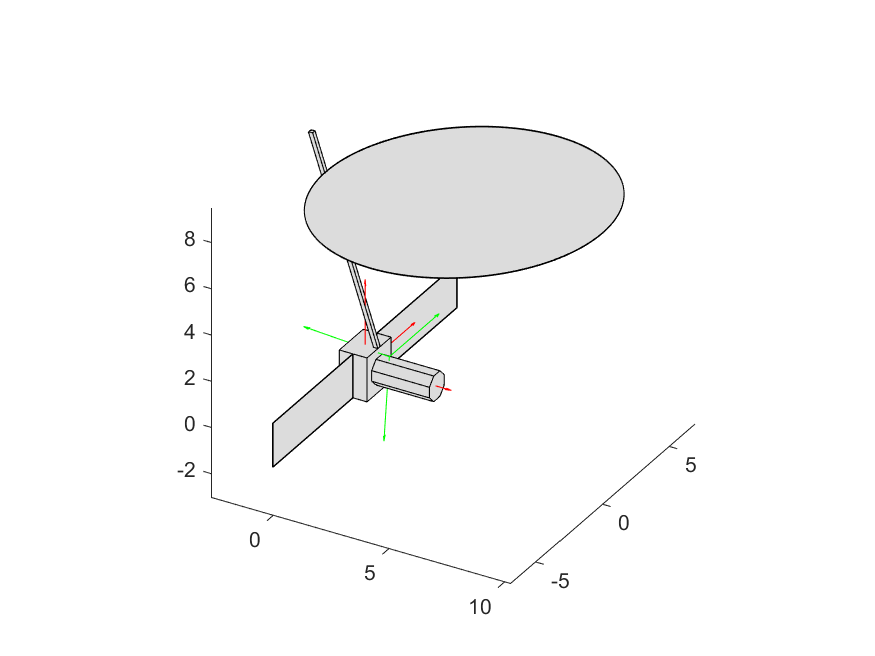
\includegraphics[scale=0.7]{Images/ps2_model.png}
\caption{Principal axes at center of mass (green) and body axes at origin (red)}
\label{fig:ps2_model}
\end{figure}